To ensure that the spherical dust modelling was correct, this phase of the project started by replicating many plots from \cite{Kataoka_2015} to ensure the models accurately replicated the behaviour of the optical properties of the scattered light. 



%
%



% ----------------------------------------------
\subsection{Dust Opacities as a Function of Observing Wavelength}
% ----------------------------------------------
The replication of Figure 1 from \cite{Kataoka_2015} is presented in Figure \ref{fig: Kataoka2015Figure1Recreation}. This figure shows how the absorption and scattering mass capacities in units of \cmsq per gram for dust grains of size \amax = 1 \micron and 100 \micron change with observing wavelength. It can be concluded from this figure that for smaller dust grain (red lines, \amax = 1 \micronNS), the absorption opacity is much greater than the scattering opacity. Alternatively, for the larger dust grain (blue lines, \amax = 100 \micronNS), from roughly 0.1-2 mm ($10^2 - 2\times10^3$ \micronNS), the scattering opacity is greater than the absorption opacity. The observing wavelengths in this project range between \bseven to \bfourNS, which essentially fall within this range. This tells us that within our observing wavelengths, smaller dust grains are less efficient at scattering than large dust grains. But at the lower and upper bounds of \bseven and \bfour the scattering and absopption is relatively similar. \add{connect this back to the Pw plot}




\begin{figure*}[h]
  \centering
  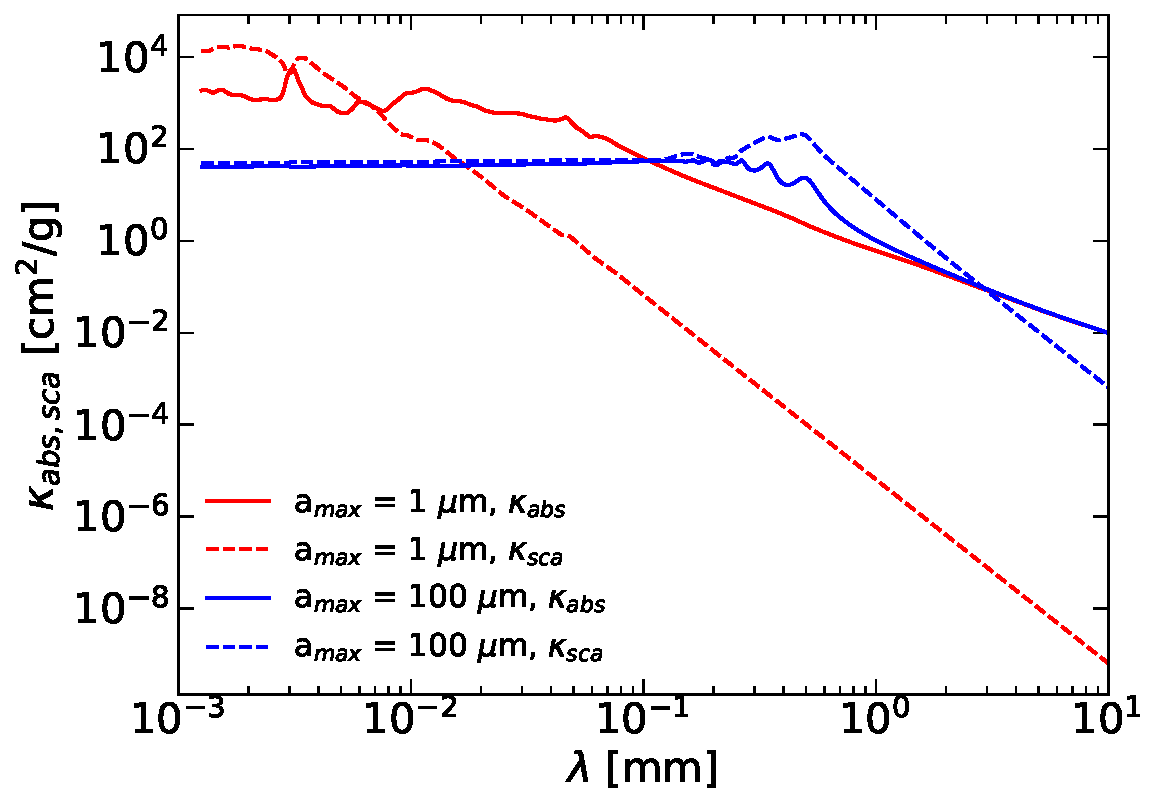
\includegraphics[width=0.6\textwidth]{WRITEUP_AND_IMAGES/IMAGES/WRITEUP/DustModels/Kataoka2015Fig1.pdf}
  \caption{Absorption and scattering mass opacities as a function of observing wavelength for grain sizes of 1\micron and 100 \micronNS. Recreation of Figure 1 from \cite{Kataoka_2015}. }
  \label{fig: Kataoka2015Figure1Recreation}
\end{figure*}
% ----------------------------------------------

% ----------------------------------------------
\subsection{Polarization Dependence on Scattering Angle}
% ----------------------------------------------
A replication of Figure 2 from \cite{Kataoka_2015} is presented in \ref{fig: Kataoka2015Figure2Recreation}. It was replicated for the four wavelengths this project is focusing on. This figure explores how polarization changes with scattering angle, and highlights how the polarization peaks at a scattering angle of for smaller dust grains (10 \micron and 100 \micronNS). Alternatively, for much larger dust grains (1 mm and 1 cm), the polarization degree remains much closer to 0, indicating that polarization from scattering is not efficient at larger grains. 



\begin{figure*}[h]
  \centering
  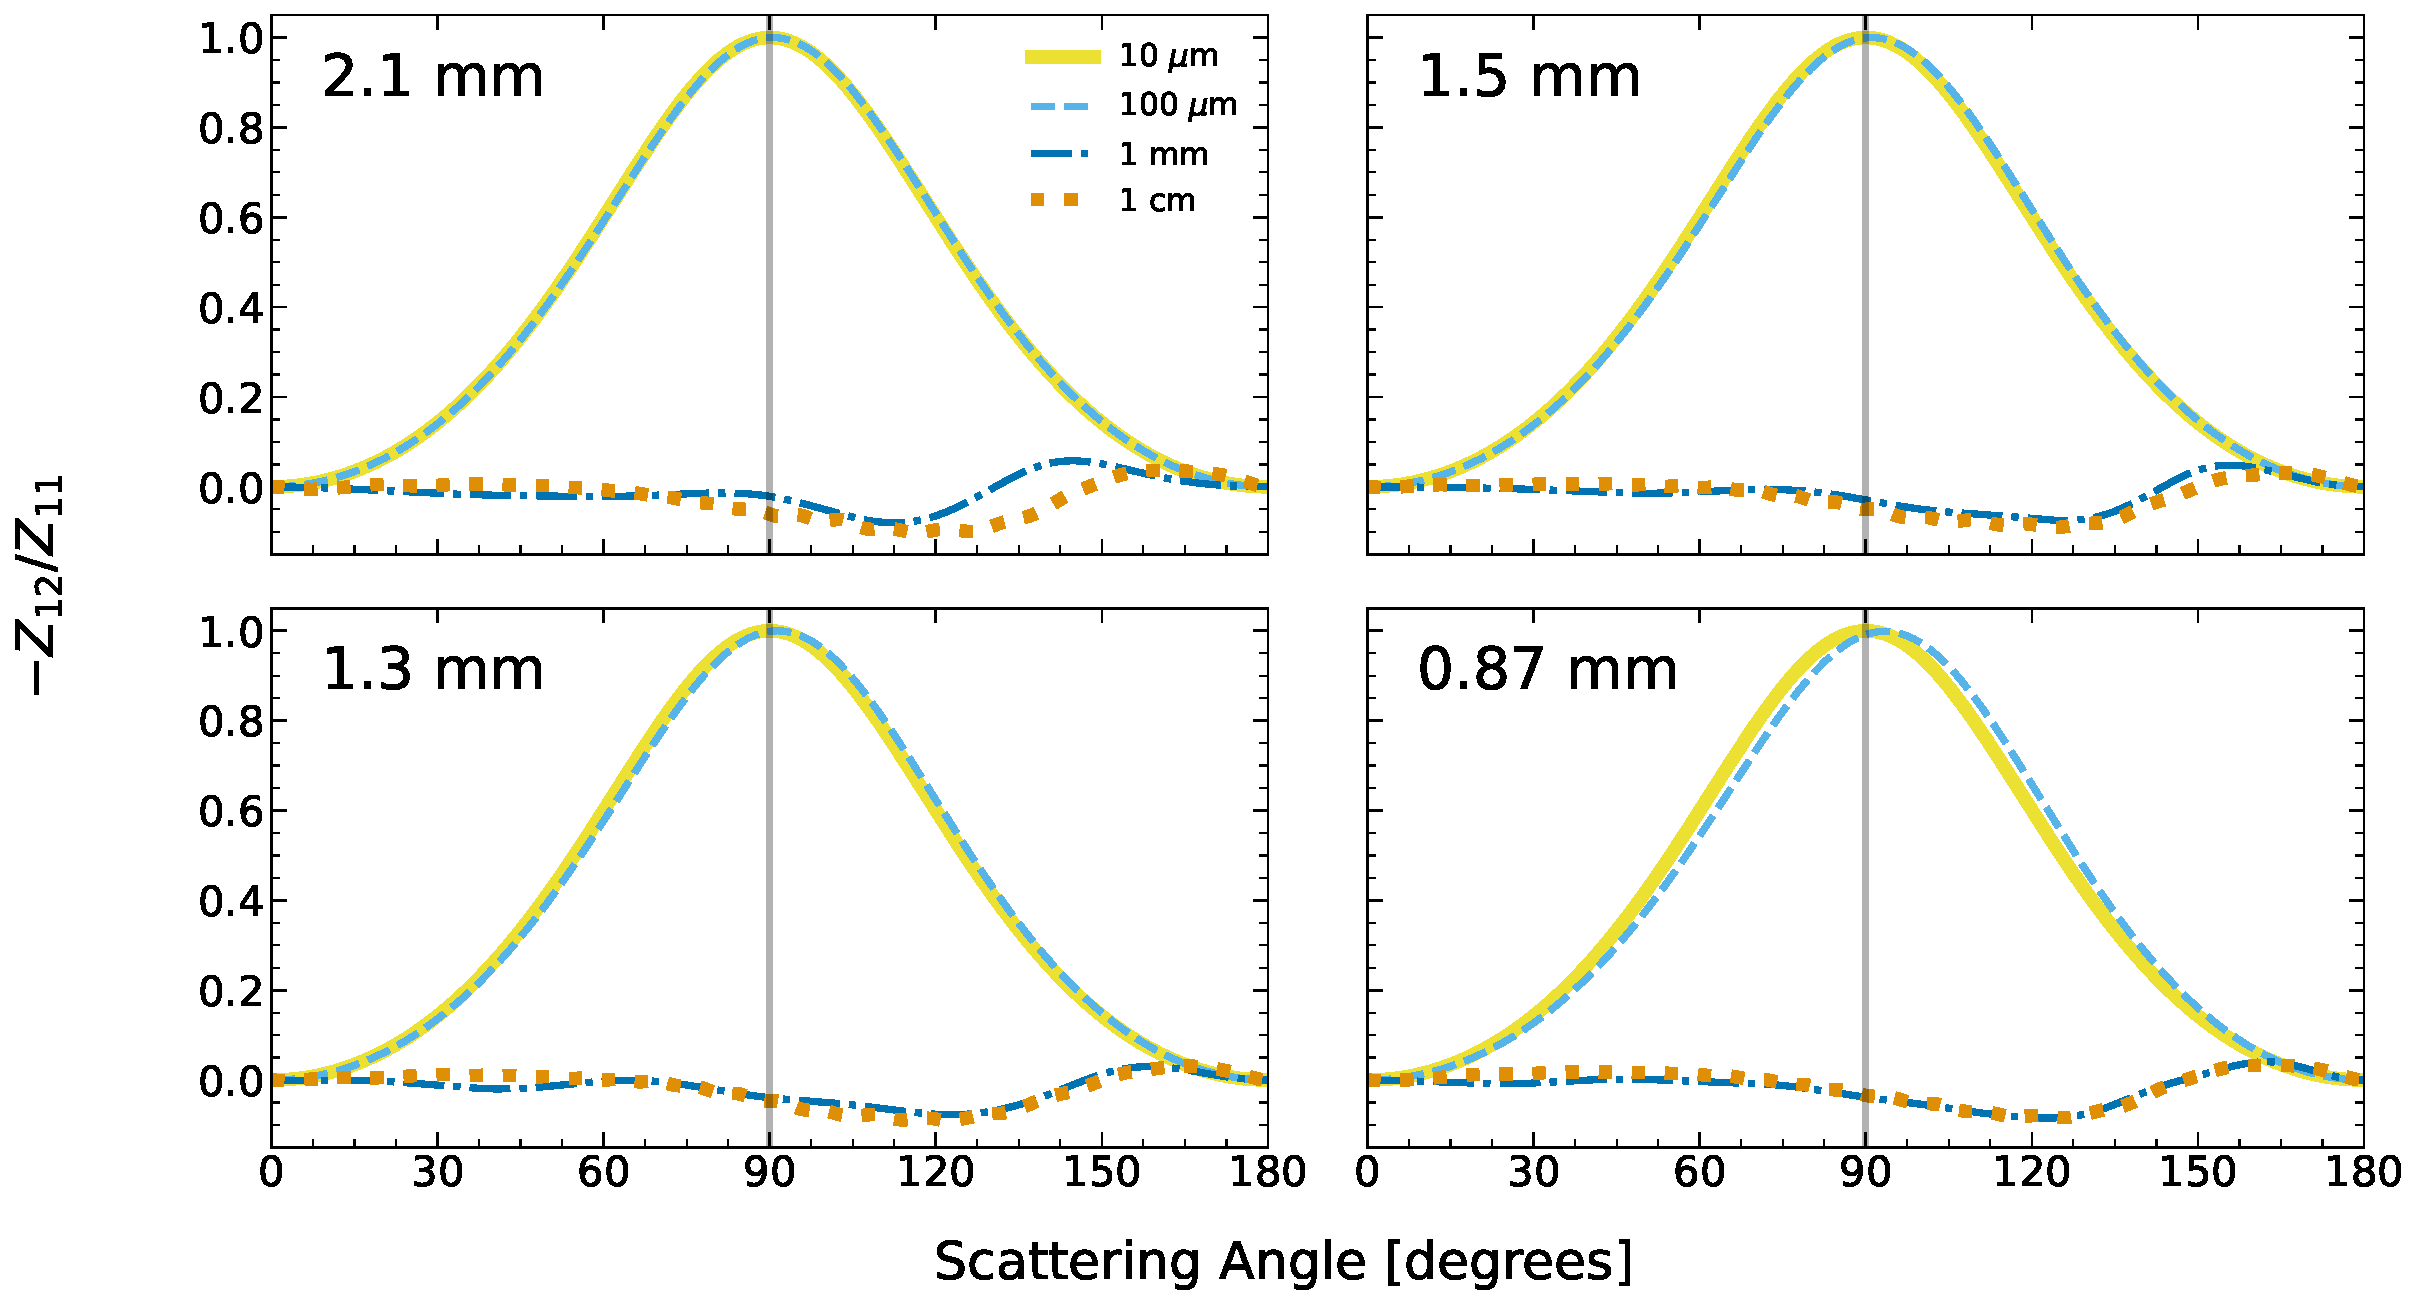
\includegraphics[width=1.1\textwidth]{WRITEUP_AND_IMAGES/IMAGES/WRITEUP/DustModels/Kataoka2015Fig2_grid.pdf}
  \caption{Degree of polarization as a function of scattering angle for maximum grain sizes of 10 \micronNS, 100 \mironNS, 1 mm and 1 cm. This is a replication of Figure 2 from \cite{Kataoka_2015}.}
  \label{fig: Kataoka2015Figure2Recreation}
\end{figure*}

% ----------------------------------------------






% ----------------------------------------------
\subsection{Polarization and Albedo as a Function of Grain Size}
% ----------------------------------------------
In Figure \ref{fig: Kataoka2015Figure3Recreation}, Figure 3 from \cite{Kataoka_2015} was recreated for the four wavelengths from this project. The figure shows how polarization and albedo change with grain size. The main idea is that polarization is much more efficient for smaller grains, and quickly drops off as the dust grains get large. Alternatively, the albedo (scattering) is much more efficient for larger grains, as there is more surface area for the light to reflect off of. Additionally, a grey line is added at the characteristic grain size. We expect the polarization from scattering to peak at this value for each wavleength, which is what is observed. 


\begin{figure*}[h]
  \centering
  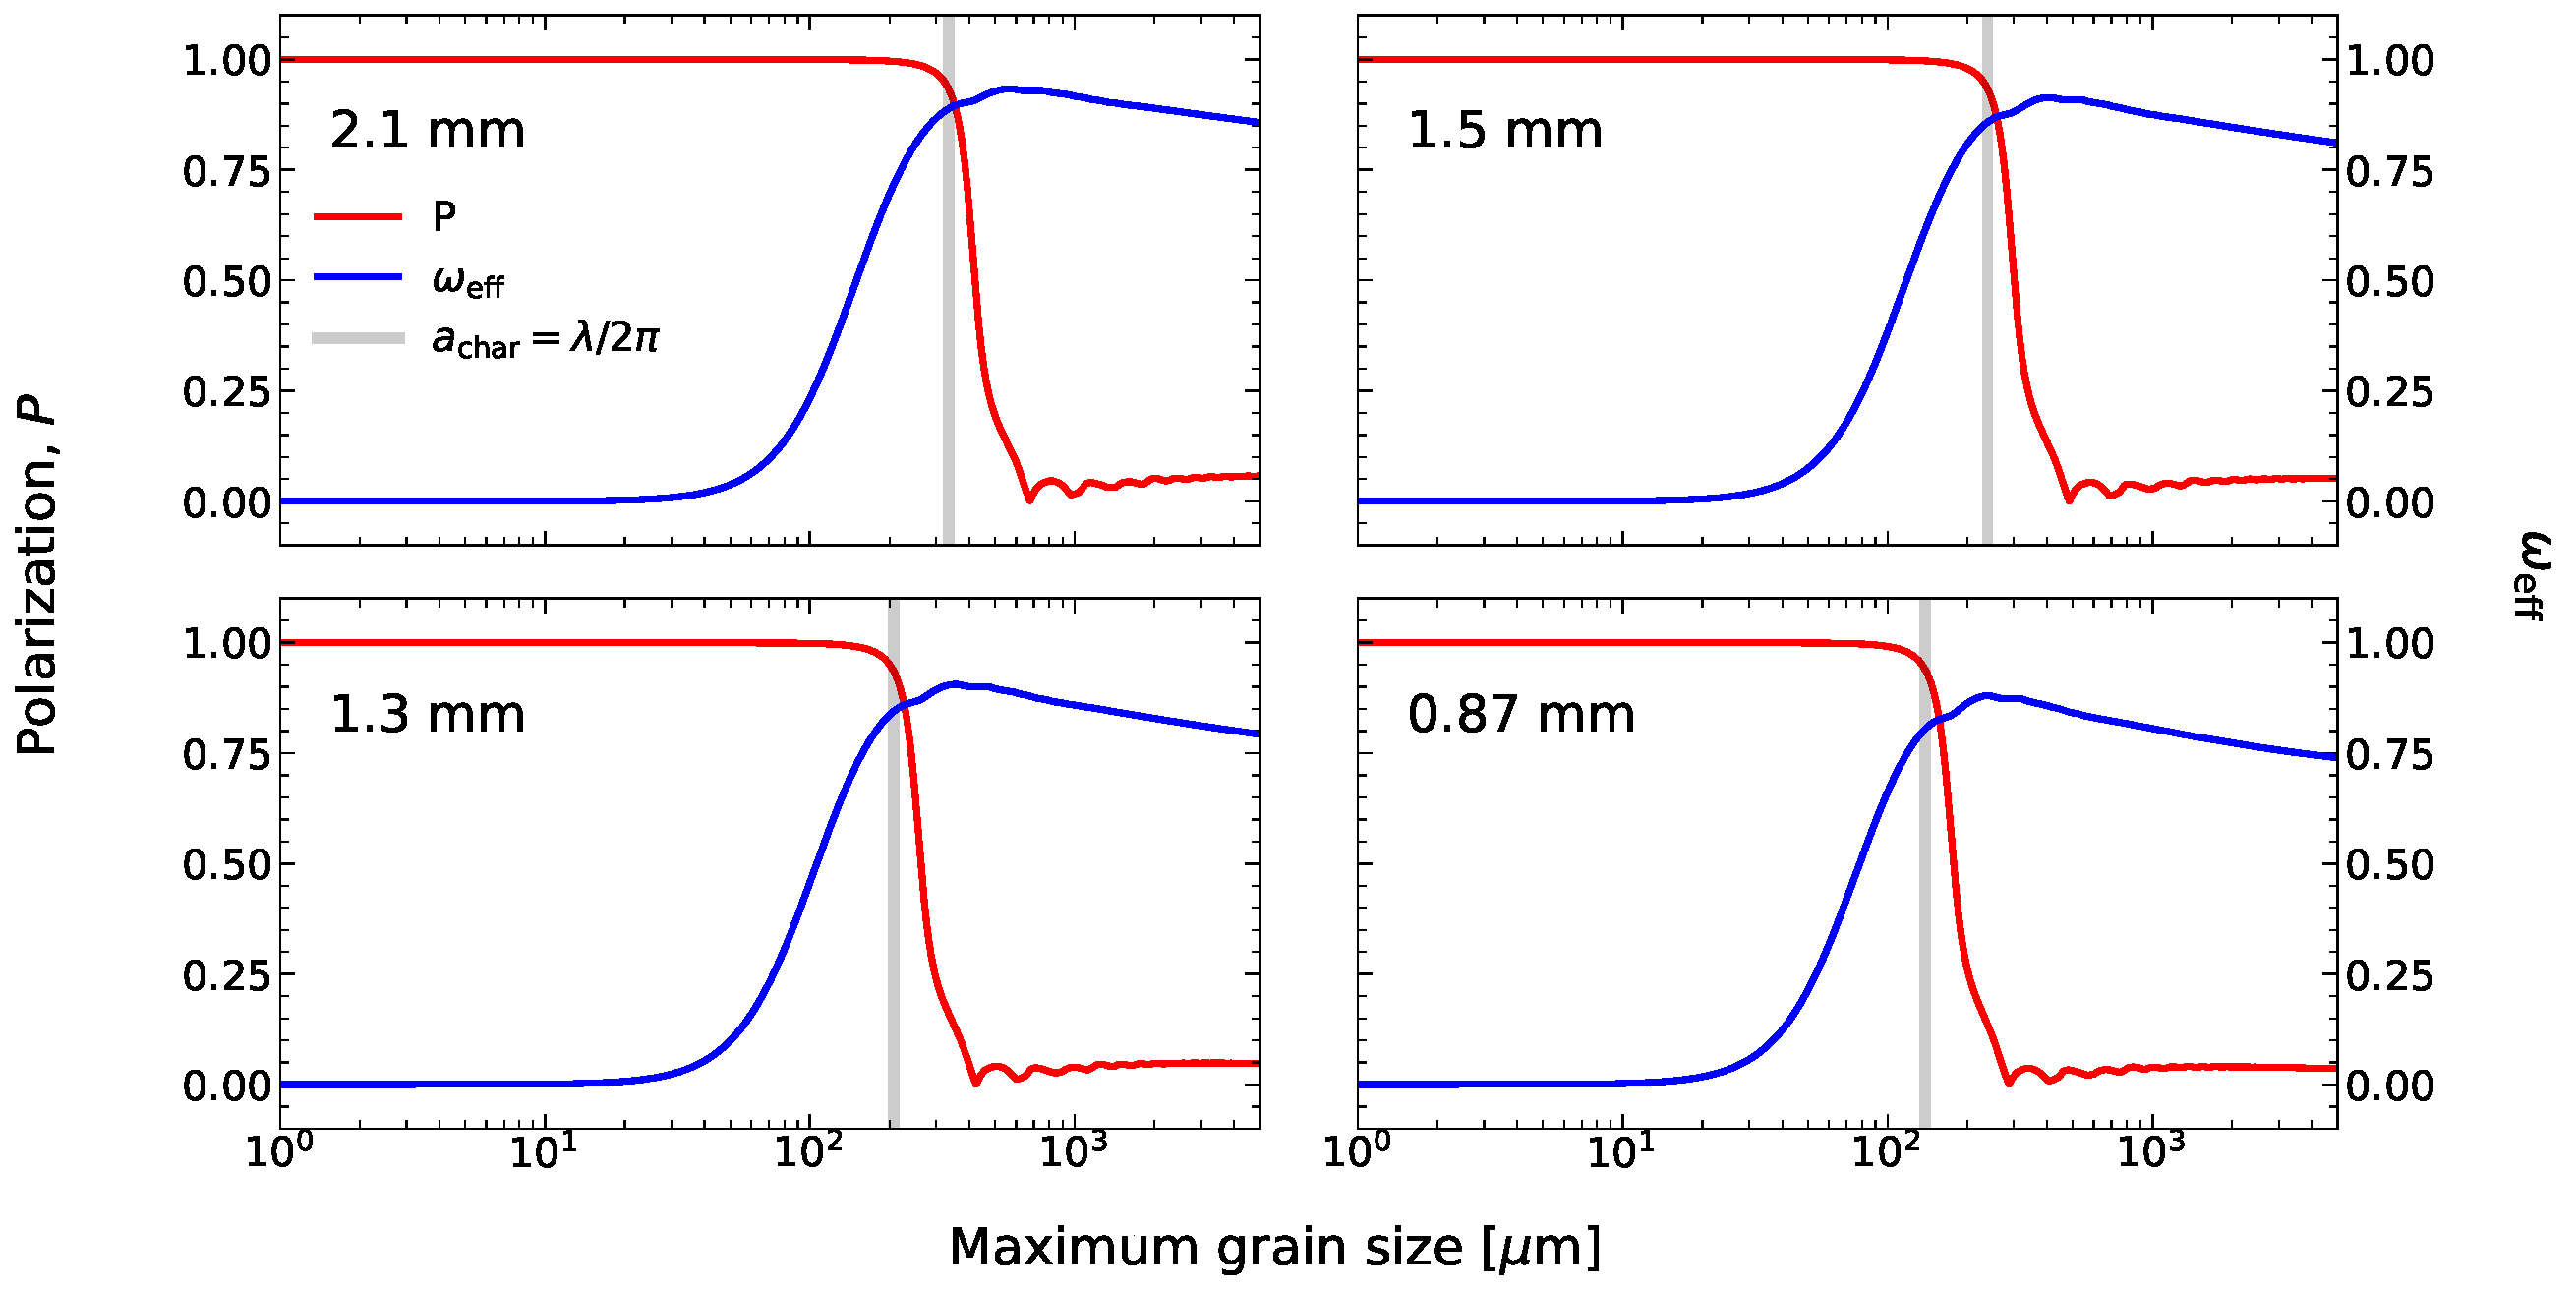
\includegraphics[width=1.1\textwidth]{WRITEUP_AND_IMAGES/IMAGES/WRITEUP/DustModels/P_vs_w_eff_vs_grainsize_grid_smooth.pdf}
  \caption{Plot of polarization $P$ in red and effective albedo as in blue a function of grain size. \question{Make this one row to take up less space or will that be too small?}. The characteristic grain size for each wavelength is overplotted in grey, highlighting that is roughly correcponts to the local maximima of both curves. This is a recreation of Figure 3 from \cite{Kataoka_2015}.}
  \label{fig: Kataoka2015Figure3Recreation}
\end{figure*}

% ----------------------------------------------



% ----------------------------------------------
\subsection{$\mathbf{P\omega}$ as a Function of Grain Size}
% ----------------------------------------------
Figure \ref{fig: Pw_vs_grainsize} is a replication of Figure 4 from \cite{Kataoka_2015} for the observing wavelengths this project focuses on. This figure explores \Pw as a function of grain size, which is similar to \ref{fig: Kataoka2015Figure3Recreation}, but with both lines being multiplied together rather than plotted separately. This plot highlights the polarized scattering efficiency, which peaks at roughly the characteristic grain size, which is plotted with a dashed line in the respective colour. 

This plot shows that we expect to be able to detect grain sizes on the order of hundreds of microns. As discussed in Chapter \ref{sec: intro_mw}, using multi-wavelength observations allows us to simultaneously fit all wavelengths to place a better constraint on the grain size. How this is done is explained in Chapter \ref{sec: ch5_determining_abest}. 



% ------------------------------------------------------
\begin{table}[h!]
\centering
\caption{Maximum grain size corresponding to the peak $P\omega$ value, and characteristic grain size as a dashed line for each wavelength in Figure \ref{fig: Pw_vs_grainsize}.}
\label{tab:amax_peak_values}
\begin{tabular}{lcccc}
\toprule
\textbf{Parameter} & \textbf{\bfour} & \textbf{\bfive} & \textbf{\bsix} & \textbf{\bseven} \\
\midrule
$a_{\max}$ (\micronNS)
& 307.88
& 223.71
& 196.46
& 134.50 \\

$a_{\text{char}}$ (\micronNS)
& 334.23
& 238.73
& 206.90
& 138.46 \\

\bottomrule
\end{tabular}
\label{tab: amax_peak_values}
\end{table}
% ------------------------------------------------------




\begin{figure*}[h]
  \centering
  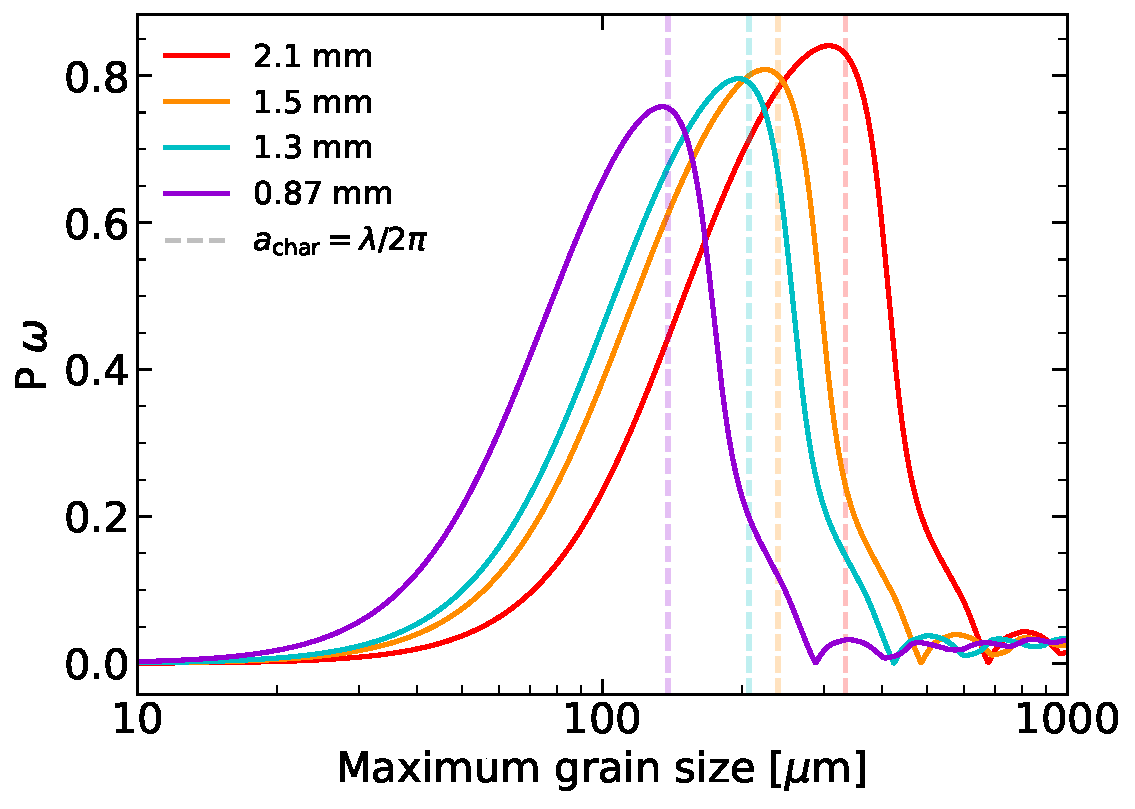
\includegraphics[width=0.75\textwidth]{WRITEUP_AND_IMAGES/IMAGES/WRITEUP/DustModels/Pw_vs_grainsize_smooth.pdf}
  \caption{Polarization curves (\PwNS) versus grain size for each wavelength. Over-plotted as a dashed line with matching colour is the characteristic grain size. This is a recreation of Figure 4 from \cite{Kataoka_2015}}
  \label{fig: Pw_vs_grainsize}
\end{figure*}
% ----------------------------------------------



\noindent \question{Zhang plots?}



\noindent \question{Should I add a section about replicating plots from glitterin?}
